\chapter{Literature Review}
\label{sec:literature_review}

\section{Mobile Communications}
\begin{German}
    \textbf{Mobilfunk} ist ein Teilbereich der Telekommunikation, der sich mit der drahtlosen Übertragung von Sprache und Daten über Funknetze befasst. Die Planung dieser Netze wird als \textbf{Mobilfunkplanung} bezeichnet. Innerhalb dieses Fachgebiets haben sich unterschiedliche Disziplinen entwickelt:

    \begin{itemize}
        \item \textbf{Netzwerkplanung:} Die Netzwerkplanung umfasst die Umsetzung und Optimierung der Netzwerkarchitektur eines Mobilfunknetzes. Sie beinhaltet die detaillierte Planung der Zellstruktur, Frequenzverteilung, Kapazitätsberechnung und Interferenzminimierung, um eine effiziente, stabile und leistungsfähige Netzabdeckung sicherzustellen. Ein wesentlicher Bestandteil der Netzwerkplanung ist die Bestimmung des geografischen Perimeters, in dem eine Mobilfunkanlage erforderlich ist.
        Der Schwerpunkt der Netzwerkplanung liegt auf elektronischen und signaltechnischen Aspekten, wodurch sie stark standardisiert und international reguliert ist. Aufgrund dieser Standardisierung und technischen Komplexität ist die verfügbare Fachliteratur zur Mobilfunkplanung weitgehend auf die Netzwerkplanung fokussiert.

        \item \textbf{Standortplanung:} Die Standortplanung bezieht sich auf die Identifikation und bauliche Umsetzung eines physischen Standorts innerhalb des durch die Netzwerkplanung definierten Perimeters. Dazu gehört die Auswahl geeigneter Standorte unter Berücksichtigung von topografischen, baulichen, rechtlichen und umweltbezogenen Faktoren.
        Im Gegensatz zur Netzwerkplanung ist die Standortplanung weniger standardisiert, da sie stark von lokalen Gegebenheiten abhängt. Diese Variabilität führt dazu, dass die wissenschaftliche Fachliteratur zu diesem Thema vergleichsweise begrenzt ist. Stattdessen ergeben sich Planungsprozesse und Begriffsdefinitionen oft aus der Praxis, beispielsweise durch behördliche Richtlinien oder unternehmensinterne Prozesse.
    \end{itemize}

    Diese Arbeit konzentriert sich auf die Standortplanung von Mobilfunkanlagen. Zunächst werden die hierfür relevanten Grundlagen geschaffen, ohne dabei zu sehr auf technische Details einzugehen. In der Fallstudie wird dann noch genauer auf die einzelnen Prozesse im Zusammenhang mit BIM eingegangen.
\end{German}

\begin{English}
    \textbf{Mobile communications} is a subfield of telecommunications that deals with the wireless transmission of voice and data over radio networks. The planning of these networks is referred to as \textbf{mobile network planning}. Within this field, different disciplines have developed:

    \begin{itemize}
        \item \textbf{Network Planning:} Network planning involves the implementation and optimization of the network architecture of a mobile network. It includes detailed planning of the cell structure, frequency distribution, capacity calculation, and interference minimization to ensure efficient, stable, and high-performance network coverage. An essential part of network planning is determining the geographical perimeter where a mobile radio system is required.
        The focus of network planning is on electronic and signal engineering aspects, making it highly standardized and internationally regulated. Due to this standardization and technical complexity, the available literature on mobile network planning is largely focused on network planning.

        \item \textbf{Site Planning:} Site planning refers to the identification and construction of a physical site within the perimeter defined by network planning. This includes selecting suitable sites, taking into account topographical, structural, legal, and environmental factors.
        In contrast to network planning, site planning is less standardized, as it depends heavily on local conditions. This variability means that the scientific literature on this topic is relatively limited. Instead, planning processes and definitions often arise from practice, such as regulatory guidelines or internal company processes.
    \end{itemize}

    This work focuses on the site planning of mobile radio systems. First, the relevant basics are established without going into too much technical detail. The case study then goes into more detail on the individual processes related to BIM.
\end{English}


\subsection{International Status of Mobile Communications}
\begin{German}
    Der gesamte mobile Datenverkehr nimmt weltweit exponentiell zu. Bis ungefähr 2020 verdoppelte sich der Verkehr etwa alle zwei Jahre. Für die Zeit bis 2030 werden noch immer jährliche Wachstumsraten von durchschnittlich 19 \% prognostiziert. Derzeit werden 34 \% des mobilen Datenverkehrs über 5G-Netzwerke abgewickelt. Bis 2030 soll dieser Anteil auf 80 \% steigen.

    Zum Anstieg entscheidend beigetragen haben Video-Streaming mit immer höheren Bildschirmauflösungen (4K, 8K), das mitlerweile 74 \% des mobilen Datenverkehrs ausmacht. Haupttreiber des zukünftigen Wachstums wird besonders in den Bereichen des autonomen Fahren, Extended Reality, Industrie 4.0 sowie generativer KI gesehen. 
    Fixed Wireless Access (FWA) wird stark an bedeutung gewinnen und bis 2030 mit 36 \% einen erheblichen Anteil des Datenverkehrs ausmachen. Dabei werden stationäre Geräte (z. B. Computer) über ein CPE-Gerät mit einer festen Breitbandverbindung versorgt, die über mobile Netzwerke (4G/5G) bereitgestellt wird. Besonders in wirtschaftlich schwächer entwickelten Regionen wird FWA traditionelle Festnetzanschlüsse zunehmend als kostengünstigere Alternative verdrängen. \cite{EricssonMobilityReport}
\end{German}

\begin{English}
    The global mobile data traffic is increasing exponentially. Until around 2020, traffic volumes doubled approximately every two years. For the period up to 2030, annual growth rates of an average of 19 \% are still projected. Currently, 34 \% of mobile data traffic is handled via 5G networks. By 2030, this share is expected to rise to 80 \%.  

    A key driver of this increase has been video streaming with ever-higher screen resolutions (4K, 8K), which now accounts for 74 \% of mobile data traffic. The main drivers of future growth are expected to be in the areas of autonomous driving, extended reality, Industry 4.0, and generative AI.  
    Fixed Wireless Access (FWA) is expected to gain significant importance and account for a substantial 36 \% of total data traffic by 2030. In this context, stationary devices (e.g., computers) are supplied via a CPE device with a fixed broadband connection provided through mobile networks (4G/5G). Particularly in economically less developed regions, FWA is expected to increasingly replace traditional fixed-line connections as a more cost-effective alternative. \cite{EricssonMobilityReport}
\end{English}

\subsection{National Status of Mobile Communications}
\begin{German}
    In der Schweiz vertritt der Bund die Ansicht, dass eine leistungsfähige Telekommunikationsinfrastruktur für die Wirtschaft und Gesellschaft einen hohen Stellenwert hat. Ein rascher Ausbau leistungsfähriger 5G Netze sei deshalb wichtig. Nach Angaben der drei Betreiber sind dafür 7'500 neue Antennenstandorte und Investitionen in der Höhe von 3.2 Milliarden Franken notwendig. \cite{bundesratNachhaltigesMobilfunknetzBericht2022}

    Ihr Marktanteil nach Kundenanzahl lag Ende 2023 bei Swisscom 54.3 \%, bei Sunrise 23.6 \% und bei Salt 17.1 \% \cite{bakomMarktanteileMobilfunknetz}. Die Marktdurchdringung betrug 128.9 \%. Damit gibt es mehr aktive Simkarten als Einwohner. \cite{bakomAnzahlMobilfunkkundinnenUnd}.

    Zum Schutz der Bevölkerung vor wissenschaftlich nachgeweisenen Schäden aufgrund nichtionisierender Strahlung (NIS), hat die International Commission on Non-Ionizing Radiation Protection (ICNIRP) empfohlene Grenzwerte definiert. Diese wurden vom Bund in der Verordnung über den Schutz vor nichtionisierender Strahlung (NISV) als Immissionsgrenzwerte übernommen und entsprechen der Empfehlung der EU. Diese müssen an allen Orten eingehalten werden, an denen sich Menschen aufhalten können. Aufgrund gesundheitlicher Bedenken, wurden sogenannte Anlagegrenzwerte definiert \cite{baumannMitVerordnungUeber2005}. Dieser verschärfte Grenzwert beträgt noch 10 \% des Immissionsgrenzwert und muss an Orten mit empfindlicher Nutzung (OMEN) eingehalten werden. Dies sind Bereiche, von denen auszugehen ist, dass sich Menschen regelmässig über längere Zeit aufhalten. Die elektrische Feldstärke beträgt dort ein Zehntel des in Deutschland und Frankreich zulässigen Wertes. Die Leistung einer elektromagnetischen Welle ist dabei proprtional zum Quadrat der elektrischen Feldstärke. Eine um Faktor 10 reduzierte Feldstärke, führt damit zu einer um Faktor 100 sinkenden Sendeleistung \cite{chance5gAnlagegrenzwerteImMobilfunk}.
    Sobald eine Anlage die maximal zulässige Sendeleistung erreicht hat, kann diese nicht mehr weiter ausgebaut werden. Zur Erhöhung der Netzkapazität müssen dann neue Stanorte gebaut werden \cite{bundesratNachhaltigesMobilfunknetzBericht2022}.
\end{German}

\begin{English}
    In Switzerland, the federal government takes the view that a powerful telecommunications infrastructure is of great importance for the economy and society. Therefore, rapid expansion of powerful 5G networks is important. According to the three providers, this requires 7,500 new antenna sites and investments of CHF 3.2 billion. \cite{bundesratNachhaltigesMobilfunknetzBericht2022}

    Their market share by number of customers was 54.3 \% for Swisscom, 23.6 \% for Sunrise, and 17.1 \% for Salt at the end of 2023 \cite{bakomMarktanteileMobilfunknetz}. The market penetration was 128.9 \%. This means that there are more active SIM cards than residents. \cite{bakomAnzahlMobilfunkkundinnenUnd}.

    To protect the population from scientifically proven damage due to non-ionizing radiation (NIS), the International Commission on Non-Ionizing Radiation Protection (ICNIRP) has defined recommended limit values. These have been adopted by the federal government in the Ordinance on Protection against Non-Ionizing Radiation (NISV) as immission limit values and correspond to the EU recommendation. These must be complied with at all locations where people can be present. Due to health concerns, so-called system limit values have been defined \cite{baumannMitVerordnungUeber2005}. This stricter limit value is 10 \% of the immission limit value and must be complied with at locations with sensitive use (OMEN). These are areas where it is assumed that people will be present regularly for longer periods. The electric field strength there is one-tenth of the permissible value in Germany and France. The power of an electromagnetic wave is proportional to the square of the electric field strength. A field strength reduced by a factor of 10 thus leads to a transmission power reduced by a factor of 100 \cite{chance5gAnlagegrenzwerteImMobilfunk}. Once a system has reached the maximum permissible transmission power, it can no longer be expanded. To increase network capacity, new sites must be built. \cite{bundesratNachhaltigesMobilfunknetzBericht2022}.
\end{English}

\subsection{Mobile Network Generations}
\begin{German}
    Ungefähr alle zehn Jahre wird eine neue Mobilfunkgeneration eingeführt. Diese haben jeweils eine höhere Datenübertragungsrate, eine geringere Latenz und eine höhere Anzahl an gleichzeitig verbundenen Geräten. Bis zur Einführung der sechten Generation (6G Vision, ca. 2030) wird derzeit die fünfte Generation (5G) ausgebaut. Ebenfalls praxisrelevant ist die vierte Generation (LTE), die ab 2012 ausgebaut wurde. Die dritte Generation (UMTS) wird als erstes von Swisscom auf Ende 2025 eingestellt \cite{swisscomAbschaltung3GErneuerung}. Die zweite Generation (GSM) wurde von den drei Anbeitern zwischen 2020 und 2023 eingestellt.
\end{German}

\begin{English}
    Approximately every ten years, a new mobile network generation is introduced. Each generation has a higher data transfer rate, lower latency, and a higher number of devices connected simultaneously. Currently, the fifth generation (5G) is being expanded until the introduction of the sixth generation (6G Vision, around 2030). Also relevant in practice is the fourth generation (LTE), which was expanded from 2012. The third generation (UMTS) will be discontinued by Swisscom at the end of 2025 \cite{swisscomAbschaltung3GErneuerung}. The second generation (GSM) was discontinued by the three providers between 2020 and 2023.
    To protect the population from scientifically proven damage due to non-ionizing radiation (NIS), the International Commission on Non-Ionizing Radiation Protection (ICNIRP) has defined recommended limit values. These have been adopted by the federal government in the Ordinance on Protection against Non-Ionizing Radiation (NISV) as immission limit values and correspond to the EU recommendation. These must be complied with at all locations where people can be present. Due to health concerns, so-called system limit values have been defined \cite{baumannMitVerordnungUeber2005}. This stricter limit value is 10 \% of the immission limit value and must be complied with at locations with sensitive use (OMEN). These are areas where it is assumed that people will be present regularly for longer periods. The electric field strength there is one-tenth of the permissible value in Germany and France. The power of an electromagnetic wave is proportional to the square of the electric field strength. A field strength reduced by a factor of 10 thus leads to a transmission power reduced by a factor of 100 \cite{chance5gAnlagegrenzwerteImMobilfunk}.
    Once a system has reached the maximum permissible transmission power, it can no longer be expanded. To increase network capacity, the existing mobile network must then be expanded \cite{bundesratNachhaltigesMobilfunknetzBericht2022}.
\end{English}

\subsection{Network Architecture}
\begin{German}
    Die Netzarchitektur eines Mobilfunknetzes kann in verschiedene Komponenten oder Teilbereiche gegliedert werden:

    \begin{itemize}
        \item \textbf{Zugangsnetz:} Das Zugangsnetz umfasst die Endgeräte, die Sendeanlagen und die Funkverbindung zwischen ihnen.
        \item \textbf{Kernnetz:} Das Kernnetz verarbeitet, steuert und vermittelt die Verbindungen und ermöglicht die Anbindung an externe Netze, wie das Internet oder das Festnetz. \cite{behnkeGrundkursMobilfunkUnd2022}
        \item \textbf{Backhaul-Anbindung:} Die beiden Netze sind über die Backhaul-Anbindung verbunden, die aufgrund ihrer hohen Kapazität vorzugsweise leitungsbasiert über Glasfaser realisiert wird. In abgelegenen Gebieten kann sie jedoch auch als Richtfunkverbindung umgesetzt werden.
    \end{itemize}

    Herzstück jeder Anlage ist die \textbf{Basisstation}, die zentrale Recheneinheit zur Steuerung der Datenübertragung.  Jede Basisstation besitz zudem mindestens eine \textbf{Antenne}, über die mittels elektromagnetischen Wellen eine bidirektionale Kommunikation mit dem Endgerät erfolgt. Üblicherweise werden pro Analge drei Sektor-Antennen verwendet, die jeweils gerichtet in einen Sektor von 120 Grad abstrahlen. Bei unterschiedlichen Technologien werden diese in unterschiedlichen Ebenen angeordnet. Jeder Antennensektor definiert dabei eine \textbf{Mobilfunkzelle}. Dadurch ergibt sich ein idealisiertes, sechseckiges Grundmuster. \cite{behnkeGrundkursMobilfunkUnd2022}
\end{German}

\begin{English}
    The network architecture of a mobile network can be divided into various components or subareas:

    \begin{itemize}
        \item \textbf{Access Network:} The access network includes the end devices, the transmitting systems, and the radio connection between them.
        \item \textbf{Core Network:} The core network processes, controls, and mediates the connections and enables connections to external networks such as the Internet or the fixed network. \cite{behnkeGrundkursMobilfunkUnd2022}
        \item \textbf{Backhaul Connection:} The two networks are connected via the backhaul connection, which is preferably implemented as a line-based connection via fiber optic due to its high capacity. However, in remote areas, it can also be implemented as a microwave connection.
    \end{itemize}

    The \textbf{base station} is the central processing unit for controlling data transmission and is the heart of each system. Each base station also has at least one \textbf{antenna} through which bidirectional communication with the end device takes place via electromagnetic waves. Typically, three sector antennas are used per system, each radiating in a sector of 120 degrees. These are arranged in different planes for different technologies. Each antenna sector defines a \textbf{mobile radio cell}. This results in an idealized hexagonal basic pattern. \cite{behnkeGrundkursMobilfunkUnd2022}
\end{English}

\subsection{System Classification}
\begin{German}
    Die Klassifizierung der Anlage kann je nach Perspektive unterschiedlich erfolgen. Aus technischer Sicht ist für die Funknetzplanung eine Unterscheidung nach Zellgrösse sinnvoll. Hier wird unterschieden zwischen Makrozellen (ländliche Gebiete), Mikrozellen (städische Gebiete), Pikozellen (Indoor-Abdeckung) und Femtozellen (Privatbereich). \cite{bundesratNachhaltigesMobilfunknetzBericht2022}

    Aus bauplanerischer Sicht hat sich eine Klassifizierung nach Standorttyp etabliert:

    \begin{itemize}
        \item \textbf{Greenfield-Standort:} überwiegen in ländlichen Gebieten. Charakteristisch dafür ist ein üblicherweise zwischen 20 und 50 Meter hocher, freistehender Mast.
        \item \textbf{Rooftop-Standort:} überwiegen in besiedelten Gebieten. Charakteristisch dafür ist die Unterbringung auf einem bestehenden Gebäude.
        \begin{itemize}
            \item Ständermast [2]
            \item Fassadenmontierter Mast [3]
            \item Dachdurchdringender Mast [4]
        \end{itemize}
    \end{itemize}
\end{German}

\begin{English}
    The classification of the system can vary depending on the perspective. From a technical point of view, a distinction according to cell size is useful for radio network planning. Here, a distinction is made between macrocells (rural areas), microcells (urban areas), picocells (indoor coverage), and femtocells (private areas). \cite{bundesratNachhaltigesMobilfunknetzBericht2022}

    From a construction planning perspective, a classification according to site type has been established: 

    \begin{itemize}
        \item \textbf{Greenfield site:} predominant in rural areas. Characteristic is a usually between 20 and 50 meters high, freestanding mast.
        \item \textbf{Rooftop site:} predominant in populated areas. Characteristic is the installation on an existing building.
        \begin{itemize}
            \item Stand mast [2]
            \item Facade-mounted mast [3]
            \item Roof-penetrating mast [4]
        \end{itemize}
    \end{itemize}
\end{English}

\begin{figure}[h]
    \centering
    \includegraphics[width=1\textwidth]{dwg/site_classification.PNG}
    \caption{Site Classification}
    \label{fig:site_classification}
\end{figure}

\begin{comment}
    Unabhängig vom Anlagetyp, erfolgt für die Planung jeweils eine Standortbesichtigung. Dort werden zusammen mit dem Anlagebetreiber und dem Eigentümer die technischen Spezifikationen definiert. Es erfolgt eine Drohnenaufnahme mittels Photogrammetrie. Bei dachdurchdringten Anlagen werden die relevanten Innenbereiche mittels terrestrischem Laserscaning erfasst. Auf Basis dieser Daten wird die Anlage geplant und die nötigen Unterlagen für eine Baubewilligung erarbeitet. Diese wird bei der zuständigen Gemeindebehörden eingereicht und nach Bewilligung gebaut. Falls mit Strahlungswerten von über 80 \% der zulässigen Imissionsgrenzwert zu rechnen ist, muss vor Inbetriebnahme der Anlage noch eine Sicherheitsmessung erfolgen. Anschliessend wird die Anlage dem Netzbetreiber übergeben. \cite{behnkeGrundkursMobilfunkUnd2022}
\end{comment}






% Wie umgesetzt?

\section{Building Information Modeling (BIM)}
\begin{German}
    \textbf{Building Information Modeling (BIM)} ist in erster Linie eine Methodik zur digitalen Planung, Ausführung und Verwaltung von Bauwerken über den gesamten Lebenszyklus hinweg. In der Praxis wird BIM daher häufig als Synonym für eine modellbasierte Planung verwednet, obschon BIM über die reine 3D-Modellierung hinaus gehen kann (z.B. 4D). Zur präzisen Abgrenzung zum Werkzeug, dass diese Methodik ermöglicht, wird dieses nachfolgend \textbf{BIM-Software} genannt.
    Nachdem in der Einführung bereits die Entwicklung von BIM thematisiert wurde, werden im folgenden Kapitel die konzeptionellen Grundlagen erläutert. Dabei liegt der Fokus auf zentralen Konzepten, die für das spätere Verständnis der Anwendung in der Fallstudie relevant sein werden.
\end{German}

\begin{English}
    \textbf{Building Information Modeling (BIM)} is primarily a methodology for digitally planning, executing, and managing buildings over their entire life cycle. In practice, BIM is therefore often used as a synonym for model-based planning, although BIM can go beyond mere 3D modeling (e.g., 4D). To clearly distinguish it from the tool that enables this methodology, it will be referred to as \textbf{BIM software} in the following. 
    After the introduction already addressed the development of BIM, the following chapter will explain the conceptual basics. The focus is on central concepts that will be relevant for the later understanding of the application in the case study.
\end{English}

\subsection{Characteristics of a BIM Model}
\begin{German}
    Ein \textbf{BIM-Modell} besteht zunächst, wie das dreidimensionale \textbf{CAD-Modell} auch, aus geometrischen Daten im dreidimensionalen Raum. Zusätzlich zu den geometrischen Daten enthält das BIM-Modell jedoch weitere Informationen, die als \textbf{Attribute} bezeichnet werden. Während das CAD-Modell eine Aggregation rein geometrischer Primitive (Punkte, Linien, Flächen) darstellt, besteht das BIM-Modell aus parametrisierten Objekten. Dabei handelt es sich um intelligente \textbf{Bauteile}, die neben ihrer Geometrie auch Attribute wie Material und Kosten enthalten können. Diese Informationen müssen im CAD-Modell entweder graphisch oder textuell dargestellt werden. Zudem können Bauteile semantisch verknüpft werden, um Beziehungen zu modellieren. Dies soll an folgendem Beispiel dargestellt werden. \cite{astourLehrbuchGrundlagenBIMArbeitsmethode2022} \\
    
    \begin{itshape}
    \textbf{Beispiel Ingenieurbau}\\
    Eine Decke eines Einfamilienhauses soll um 10 cm abgesenkt werden.

    \textbf{BIM}: Im BIM-Modell wird das Bauteil \texttt{Decke} abgesenkt. Die Änderung wird automatisch in den Schal- und Bewehrungsplänen abgebildet. Die Bewehrungsliste wird automatisch aktualisiert. Die finanziellen Auswirkungen können direkt über eine Kostenberechnung ermittelt werden.

    \textbf{CAD \footnote{Moderne CAD-Systeme verfügen mittlerweile auch über halbautomatisierte Funktionen.}}: Die Decke wird im CAD-Modell abgesenkt. Die Änderung wird manuell in den Schal- und Bewehrungsplänen übertragen. Die Bew
    ehrungsliste muss manuell aktualisiert werden. Die finanziellen Auswirkungen müssen separat berechnet werden.
    \end{itshape}
\end{German}

\begin{English}
    A \textbf{BIM model} initially consists, like the three-dimensional \textbf{CAD model}, of geometric data in three-dimensional space. In addition to the geometric data, however, the BIM model contains additional information, referred to as \textbf{attributes}. While the CAD model represents an aggregation of purely geometric primitives (points, lines, surfaces), the BIM model consists of parametrized objects. These are intelligent \textbf{components} that can contain attributes such as material and costs in addition to their geometry. This information must be represented graphically or textually in the CAD model. In addition, components can be semantically linked to model relationships. This will be illustrated by the following example. \cite{astourLehrbuchGrundlagenBIMArbeitsmethode2022} \\

    \begin{itshape}
    \textbf{Example Civil Engineering}\\
    A ceiling slab of a single-family house is to be lowered by 10 cm.

    \textbf{BIM}: The component \texttt{ceiling slab} is lowered in the BIM model. The change is automatically reflected in the formwork and reinforcement plans. The reinforcement list is updated automatically. The financial implications can be determined directly via a cost calculation.

    \textbf{CAD \footnote{Modern CAD systems now also have semi-automated functions.}}: The ceiling slab is lowered in the CAD model. The change is manually transferred to the formwork and reinforcement plans. The reinforcement list must be updated manually. The financial implications must be calculated separately.
    \end{itshape}
 

\end{English}

\subsection{BIM Terminology}
\begin{German}
    Zur Bewertung und Klassifizierung von BIM-Prozessen und BIM-Modellen gibt es standardisierte Kennzahlen. Diese ermöglichen eine objektive Bewertung und erleichtern die Kommunikation zwischen den Projektbeteiligten. Die wichtigsten Kennzahlen sind:
\end{German}

\begin{English}
    Standardized metrics are available for evaluating and classifying BIM processes and BIM models. These enable an objective evaluation and facilitate communication between project participants. The most important metrics are:
\end{English}

\subsubsection{BIM Maturity Level}
\begin{German}
    Der \textbf{BIM-Reifegrad} ist ein Qualitätsmass, das beschreibt, wie systematisch und umfassend BIM in einem Unternehmen oder Projekt implementiert ist. Der Schwerpunkt liegt auf der Vernetzung von Daten, der Standardisierung sowie der Zusammenarbeit zwischen den Beteiligten. Gemäß VDI 2552 werden die folgenden vier Reifegrade unterschieden: \cite{astourLehrbuchGrundlagenBIMArbeitsmethode2022,eichlerBIMcertHandbuchGrundlagenwissen2023}\\
\end{German}
\begin{English}
    The \textbf{BIM maturity level} is a quality measure that describes how systematically and comprehensively BIM is implemented in a company or project. The focus is on data networking, standardization, and collaboration between the participants. According to VDI 2552, the following four maturity levels are distinguished: \cite{astourLehrbuchGrundlagenBIMArbeitsmethode2022,eichlerBIMcertHandbuchGrundlagenwissen2023}\\
\end{English}

\begin{table}[h]
    \centering
    \renewcommand{\arraystretch}{1.2} % Adjust row height for better readability
    \setlength{\tabcolsep}{5pt} % Adjust column spacing
    \begin{tabularx}{\textwidth}{|c|l|X|}
        \hline
        \textbf{Level} & \textbf{BIM Usage} & \textbf{Description}  \\
        \hline
        \textbf{0} & None &  Traditional 2D CAD drafting is used with no object-based modeling or intelligent data sharing. Collaboration is minimal, and document exchange is paper-based or in simple file formats. \\
        \hline
        \textbf{1} & None &  Combination of 2D and 3D CAD tools. While 3D models may be used internally, there is no standardized collaboration between different disciplines. Data exchange remains file-based without integrated workflows. \\
        \hline
        \textbf{2} & Collaborative &  Different disciplines work on their own BIM models, which are then shared and combined at specific project stages. Collaboration is structured, but data exchange is still semi-automated, requiring manual coordination. Lifecycle phases are considered separately. \\
        \hline
        \textbf{3} & Integrated & All disciplines collaborate in a fully connected and shared BIM environment. A single, integrated model covers the entire building lifecycle, from design to operation. Automated data exchange and real-time collaboration enable seamless workflows. \\
        \hline
    \end{tabularx}
    \caption{BIM Stages and Their Characteristics}
    \label{tab:BIM_stages}
\end{table}

\subsubsection{Level of Development (LOD)}

\begin{German}
    Der \textbf{Fertigstellungsgrad (LOD)} eines Modells gibt an, wie viele Projektinformationen bereits im Modell enthalten sind. Dieser setzt sich zusammen aus dem Ausarbeitungsgrad der Geometrie (LOG) und der Tiefe der alphanumerischen Information (LOI):  \\
\end{German}
\begin{English}
    The \textbf{level of development (LOD)} of a model indicates how much project information is already contained in the model. This consists of the degree of elaboration of the geometry (LOG) and the depth of the alphanumeric information (LOI):  \\
\end{English}

    \begin{equation}
        \text{LOD} = \text{LOG} + \text{LOI}
    \end{equation}
    
 \begin{German}   
    Der LOD gibt somit den Fertigstellungsgrad eines Modells zu einer bestimmten Projektphase an. Dieser wird mit Zahlen zwischen 100 und 500 gekennzeichnet (vgl. \ref{fig:Level_of_Development}). Dabei nimmt der Detailierungsgrad mit steigender Zahl zu. Mit fortschreitendem Planungsstand nimmt der LOD in der Regel zu. Da ein hoher LOD mit einem höheren Arbeitsaufwand verbunden ist, ist es wichtig zu bestimmen, wie viele Details zu welchem Zeitpunkt sinvoll sind. Dies wird mit dem Level of Information Need (LOIN) angegeben. \cite{astourLehrbuchGrundlagenBIMArbeitsmethode2022}
\end{German}
\begin{English}
    The LOD thus indicates the level of completion of a model at a specific project phase. This is marked with numbers between 100 and 500 (see \ref{fig:Level_of_Development}). The level of detail increases with increasing number. As the planning progresses, the LOD usually increases. Since a high LOD is associated with a higher workload, it is important to determine how many details are useful at what time. This is indicated by the Level of Information Need (LOIN). \cite{astourLehrbuchGrundlagenBIMArbeitsmethode2022}
\end{English}

    % Insert a picture
    \begin{figure}[h]
        \centering
        \includegraphics[width=1\textwidth]{images/bim_levels_of_development.png}
        \caption{Level of Development (LOD) \cite{ncircletechBIMLevelDevelopment}}
        \label{fig:Level_of_Development}
    \end{figure}

\subsubsection{BIM Dimensions}
\begin{German}
    Die \textbf{BIM-Dimension} beschreibt die Informationstiefe der Attribute. Sie wird angegeben durch einen Wert zwischen 3D bis 7D. Dabei nimmt der Detailierungsgrad mit steigender Zahl zu. \cite{mayBIMImImmobilienbetrieb2022}
\end{German}
\begin{English}
    The \textbf{BIM dimension} describes the depth of information of the attributes. It is indicated by a value between 3D and 7D. The level of detail increases with increasing number. \cite{mayBIMImImmobilienbetrieb2022}
\end{English}

% table
\begin{table}[h]
    \centering
    \renewcommand{\arraystretch}{1.2} % Adjust row height for better readability
    \setlength{\tabcolsep}{5pt} % Adjust column spacing
    \resizebox{\textwidth}{!}{ % Resizes table to fit within text width
    \begin{tabular}{|c|l|l|}
        \hline
        \textbf{Dimension} & \textbf{Additional Attributes} & \textbf{Use Cases} \\
        \hline
        \textbf{3D} & None & Geometric modeling \\
        \hline
        \textbf{4D} & Time & Construction scheduling, project phases \\
        \hline
        \textbf{5D} & Cost & Quantity takeoff, pricing, budgeting \\
        \hline
        \textbf{6D} & Efficiency \& Sustainability & Energy performance, lifecycle assessment \\
        \hline
        \textbf{7D} & Facility management & Operations, maintenance, asset tracking \\
        \hline
    \end{tabular}
    }
    \caption{BIM Dimensions and Information Depth}
    \label{tab:BIM_dimensions}
\end{table}

\subsubsection{BIM Types}
\begin{German}
    BIM-Anwendungsformen werden in der Ausprägung hinsichtlich zwier Dimensionen unterschieden: \cite{astourLehrbuchGrundlagenBIMArbeitsmethode2022}
    
    \begin{enumerate}
        \item \textbf{Eingriffstiefe:} Quantitätsmass, das beschreibt, inwieweit ein BIM-Modell in die Wertschöpfungskette integriert ist. Eine geringe Eingriffstiefe liegt vor, wenn BIM nur in einer einzelnen Phase genutzt wird. Eine hohe Eingriffstiefe bedeutet, dass BIM über den gesamten Lebenszyklus hinweg eingesetzt wird.
        \item \textbf{Herstellerunabhängigkeit:} Qualitätsmass der Interoperabilität, also der Fähigkeit, BIM-Modelle und Daten ausserhalb von bestimmten Softwarefamilien oder Anbietern zu nutzen.
    \end{enumerate}

    Durch die Ausprägung der beiden Dimensionen ergeben sich die folgenden vier BIM-Typen: 
\end{German}

\begin{English}
    BIM application forms are distinguished in terms of two dimensions: \cite{astourLehrbuchGrundlagenBIMArbeitsmethode2022}
    
    \begin{enumerate}
        \item \textbf{Depth of Integration:} Quantity measure that describes the extent to which a BIM model is integrated into the value chain. A low depth of integration exists when BIM is only used in a single phase. A high depth of integration means that BIM is used throughout the entire life cycle.
        \item \textbf{Software Independence:} Quality measure of interoperability, i.e., the ability to use BIM models and data outside of specific software families or providers.
    \end{enumerate}

    The following four BIM types result from the expression of the two dimensions:
\end{English}

\begin{figure}[h]
    \centering
    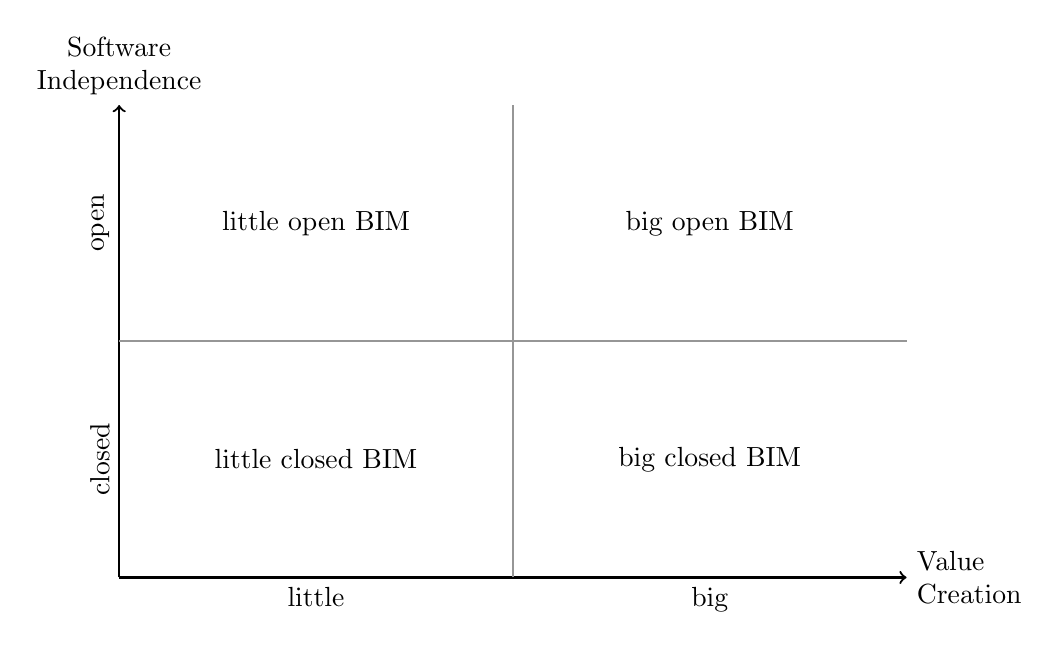
\begin{tikzpicture}

        % Define Axis Styles
        \draw[thick,->] (0,0) -- (10,0) node[anchor=west, align=left] {Value \\ Creation};
        \draw[thick,->] (0,0) -- (0,6) node[anchor=south, align=center] {Software \\ Independence};
        \node[anchor=north] at (2.5,0) {little};
        \node[anchor=north] at (7.5,0) {big};
        \node[anchor=south, rotate=90] at (0,1.5) {closed};
        \node[anchor=south, rotate=90] at (0,4.5) {open};

        % Draw Quadrant Lines
        \draw[thick, color={rgb,255:red,150; green,150; blue,150}] (5,0) -- (5,6); % Vertical
        \draw[thick, color={rgb,255:red,150; green,150; blue,150}] (0,3) -- (10,3); % Horizontal

        % Labels for quadrants
        \node at (2.5,4.5) {little open BIM};
        \node at (7.5,4.5) {big open BIM};
        \node at (2.5,1.5) {little closed BIM};
        \node at (7.5,1.5) {big closed BIM};

    \end{tikzpicture}
    \caption{BIM Types}
\end{figure}

\subsection{BIM Management}
\begin{German}
    Das \textbf{BIM-Management} beinhaltet die strategische und operative Steuerung von BIM. Es sollen damit Workflows standardisiert und die Zusammenarbeit verbessert werden. In diesem Unterkapitel sollen drei Werkzeuge vorgestellt werden (vgl. \ref{fig:BIM_management}), auf die in der Fallstudie zurückgegriffen wird.
\end{German}
\begin{English}
    \textbf{BIM management} involves the strategic and operational control of BIM. The aim is to standardize workflows and improve collaboration. In this subchapter, three tools will be presented (see \ref{fig:BIM_management}), which will be used in the case study.
\end{English}

\subsubsection{Exchange Information Requirements (EIR)}
\begin{German}
    Die \textbf{Auftraggeber-Informations-Anforderungen (AIA)} entsprechen einem auf BIM zugeschnittenen Lastenheft. Sie beschreiben, warum welche Information wann benötigt werden. Sie definieren die Anforderungen des Auftraggebers an BIM-Prozesse, Daten und Zusammenarbeit über den gesamten Projektlebenszyklus. Dazu gehören Vorgaben zu Modellstruktur, Detaillierungsgrad, Datenaustauschformaten, Verantwortlichkeiten und Kollaborationsmethoden. \cite{astourLehrbuchGrundlagenBIMArbeitsmethode2022}
\end{German}
\begin{English}
    The \textbf{Exchange Information Requirements (EIR)} correspond to a specification tailored to BIM. They describe why which information is needed when. They define the client's requirements for BIM processes, data, and collaboration throughout the entire project life cycle. This includes specifications for model structure, level of detail, data exchange formats, responsibilities, and collaboration methods. \cite{astourLehrbuchGrundlagenBIMArbeitsmethode2022}
\end{English}

\subsubsection{BIM Execution Plan (BEP)}
\begin{German}
    Der \textbf{BIM-Abwicklungsplan (BAP)} entspricht einem auf BIM zugeschnittenen Pflichtenheft. Er beschreibt, wie die Anforderungen aus dem \textbf{Auftraggeber-Informations-Anforderungen (AIA)} vom Auftragnehmer im Projekt umgesetzt werden. \cite{astourLehrbuchGrundlagenBIMArbeitsmethode2022}
\end{German}
\begin{English}
    The \textbf{BIM Execution Plan (BEP)} corresponds to a specification tailored to BIM. It describes how the requirements from the \textbf{Employer's Information Requirements (EIR)} are implemented by the contractor in the project. \cite{astourLehrbuchGrundlagenBIMArbeitsmethode2022}
\end{English}

\subsubsection{BIM Modeling Guidelines}
\begin{German}
    Die \textbf{BIM-Modellierungsrichtlinien} legen fest, wie ein BIM-Modell aufgebaut und strukturiert sein soll. Dafür werden Standards, Methoden und Anforderungen für die Erstellung und Verwaltung definiert. Sie sorgen für einheitliche Datenstrukturen, bessere Zusammenarbeit und eine hohe Modellqualität. Typischerweise werden die Modelleriungsrichtlinien im BAP definiert oder referenziert. \cite{astourLehrbuchGrundlagenBIMArbeitsmethode2022}
\end{German}
\begin{English}
    The \textbf{BIM modeling guidelines} define how a BIM model should be structured and organized. For this purpose, standards, methods, and requirements for creation and management are defined. They ensure uniform data structures, better collaboration, and high model quality. Typically, the modeling guidelines are defined or referenced in the BEP. \cite{astourLehrbuchGrundlagenBIMArbeitsmethode2022}
\end{English}

\begin{figure}[h]
    \centering
    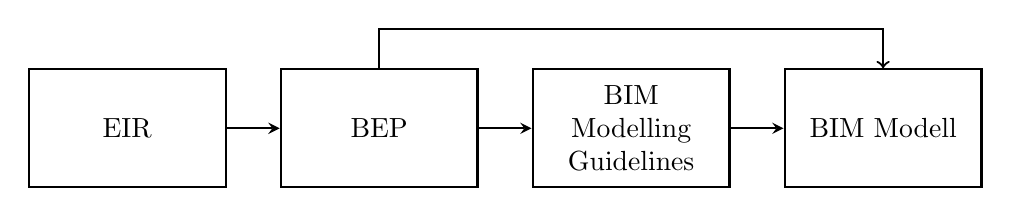
\begin{tikzpicture}[
        node distance=3.2cm, % Distance between nodes
        every node/.style={draw, minimum width=2.5cm, minimum height=1.5cm, align=center}, % Box styling
        every path/.style={thick, -stealth} % Arrow styling
        ]
        
        % Define nodes
        \node (EIR) {EIR};
        \node (BEP) [right of=EIR] {BEP};
        \node (Modelling) [right of=BEP] {BIM \\ Modelling \\ Guidelines};
        \node (BIM) [right of=Modelling] {BIM Modell};

        % Draw arrows
        \draw (EIR) -- (BEP);
        \draw (BEP) -- (Modelling);
        \draw (Modelling) -- (BIM);
        
        % Draw additional curved arrow from EIR to BIM Modell
        \draw[->] (BEP.north) |- ([yshift=0.5cm] BIM.north) -| (BIM.north);

    \end{tikzpicture}
    \caption{Simplified BIM Management Process Flow}
    \label {fig:BIM_management}
\end{figure}

\section{Scan-to-BIM}
\begin{German}
    Umbauprojekte werden in der Schweizer Bauwirtschaft immer wichtiger. Die Bauausgaben für Neubauten sind gegenüber 1980 beinahe gleich geblieben. Die Investitionen in Umbauten, Erweiterungen und Abbrüche hat sich in der gleichen Periode über verdreifacht \cite{bundesamtfuerstatstikBauausgabenNachArt}. Damit betragen die gesamtschweizerischen Investitionen für Umbauten, Erweiterungen und Abbrüchen bereits 66 \% jener für Neubauten. 

    Gleichzeitig ist bei privaten Bestandsbauten die Dokumentation häufig lückenhaft \cite{dewolfCircularBuiltEnvironmentg, kadenLeitfadenGeodaesieUnd}. Besonders ältere Gebäude verfügen oft nur über unvollständige oder veraltete Planunterlagen. Zwar lassen sich in Gemeindearchiven häufig Baueingabepläne auffinden, diese dokumentieren jedoch den ursprünglichen Bauzustand, sind oft überholt und in niedrigem Detailierungsgrad.
    
    In der Schweiz wurden 81,5 \% der Gebäude vor der Jahrtausendwende errichtet \cite{bundesamtfuerstatstikBauperiode}. Falls Planunterlagen existieren, liegen diese meist ausschließlich in Papierform vor. Doch selbst bei neueren Gebäuden sind editierbare CAD- oder BIM-Dateien meist nicht verfügbar. Nach Schweizer Recht verbleibt das Urheberrecht an Plänen beim jeweiligen Planer. Die häufig vertraglich einbezogene SIA 102 gewährt dem Bauherrn zwar das Recht auf Kopien der Arbeitserzeugnisse, doch ohne explizite vertragliche Regelung genügen bereits Papierpläne oder PDF-Dateien zur Erfüllung dieser Verpflichtung \cite{bundschwBauenRechtenUnd}. Da Planer editierbare Daten aufgrund von Haftungsrisiken nur ungern herausgeben und Bauherren sich in den meisten Fällen mit Papier- oder PDF-Plänen zufriedengeben, wird auf eine weitergehende Regelung oft verzichtet. 
    
    Dies hat zur Folge, dass selbst bei neueren Bauwerken keine digital weiterverarbeitbaren Planungsunterlagen vorliegen, was die digitale Bestandsdokumentation erheblich erschwert. Für eine modellbasierte Planung sind daher Methoden erforderlich, die den physischen Bauzustand zuverlässig in ein BIM-Modell überführen können. Eine Möglichkeit besteht darin, das Modell manuell aus vorhandenen Bauplänen zu rekonstruieren. Dieser Ansatz ist jedoch zeitaufwändig und fehleranfällig, insbesondere wenn die Pläne unvollständig oder veraltet sind. Eine effizientere Lösung stellt \textbf{Scan-to-BIM} dar. Es handelt sich um einen Prozess, bei dem ein physisches Bauwerk mithilfe von Reality-Capture-Technologien wie 3D-Laserscanning oder Photogrammetrie präzise erfasst und in ein BIM-Modell überführt wird. Dies ermöglicht eine exakte digitale Repräsentation des Ist-Zustands und bildet eine verlässliche Grundlage einer weiteren Planung.
    
    Die in der Literatur beschriebenen Scan-to-BIM-Frameworks lassen sich in verschiedene Teilprozesse unterteilen. Die Anzahl und Bezeichnung dieser Teilprozesse variieren je nach gewähltem Detaillierungsgrad, folgen jedoch einer ähnlichen Grundstruktur. Im Folgenden sollen vier zentrale Teilprozesse (vgl. \ref{fig:Scan_to_BIM_framework}) vorgestellt werden.
\end{German}

\begin{English}
    Renovation projects are becoming increasingly important in the Swiss construction industry. The construction expenditure for new buildings has remained almost the same since 1980. In the same period, investments in renovations, extensions, and demolitions have more than tripled \cite{bundesamtfuerstatstikBauausgabenNachArt}. This means that the total Swiss investments for renovations, extensions, and demolitions already amount to 66 \% of those for new buildings.

    At the same time, the documentation of private existing buildings is often incomplete \cite{dewolfCircularBuiltEnvironmentg, kadenLeitfadenGeodaesieUnd}. Older buildings, in particular, often have only incomplete or outdated planning documents. Although building permit plans can often be found in municipal archives, these document the original construction status, are often outdated, and in low detail.
    
    In Switzerland, 81.5 \% of buildings were built before the turn of the millennium \cite{bundesamtfuerstatstikBauperiode}. If planning documents exist, they are usually only available in paper form. However, even in newer buildings, editable CAD or BIM files are usually not available. According to Swiss law, the copyright to plans remains with the respective planner. Although the often contractually included SIA 102 grants the client the right to copies of the work products, paper plans or PDF files are sufficient to fulfill this obligation without explicit contractual regulation \cite{bundschwBauenRechtenUnd}. Since planners are reluctant to provide editable data due to liability risks and clients are usually satisfied with paper or PDF plans, further regulation is often dispensed with.
    
    As a result, even in newer buildings, there are no digitally processable planning documents available, which significantly complicates digital inventory documentation. For model-based planning, methods are therefore required that can reliably transfer the physical construction status into a BIM model. One possibility is to manually reconstruct the model from existing construction plans. However, this approach is time-consuming and error-prone, especially if the plans are incomplete or outdated. A more efficient solution is \textbf{Scan-to-BIM}. It is a process in which a physical building is precisely captured using reality capture technologies such as 3D laser scanning or photogrammetry and transferred into a BIM model. This enables an exact digital representation of the actual state and provides a reliable basis for further planning.
    
    The Scan-to-BIM frameworks described in the literature can be divided into various sub-processes. The number and designation of these sub-processes vary depending on the chosen level of detail but follow a similar basic structure. In the following, four central sub-processes (see \ref{fig:Scan_to_BIM_framework}) will be presented.
\end{English}

\begin{figure}[h]
    \centering
    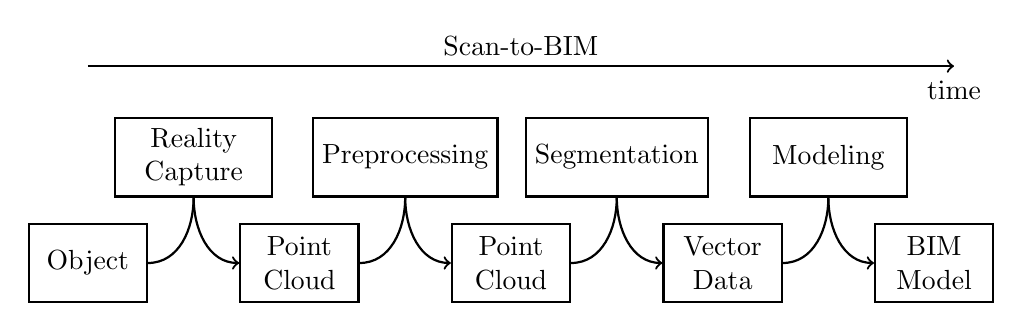
\begin{tikzpicture}[
        node distance=1.9cm, % Distance between nodes
        object/.style={draw, minimum width=1.5cm, minimum height=1cm, align=center}, % Box styling
        process/.style={draw, minimum width=2cm, minimum height=1cm, align=center}, % Box styling
        every path/.style={thick, -stealth} % Arrow styling
        ]
        
        % Define nodes
        \node (object) [object] {Object};
        \node (RC) [process, above right of=object] {Reality \\ Capture};
        \node (pointcloud1) [object, below right of=RC] {Point \\ Cloud};
        \node (PP) [process, above right of=pointcloud1] {Preprocessing};
        \node (pointcloud2) [object, below right of=PP] {Point \\ Cloud};
        \node (Segmentation) [process, above right of=pointcloud2] {Segmentation};
        \node (vector) [object, below right of=Segmentation] {Vector \\ Data};
        \node (Modeling) [process, above right of=vector] {Modeling};
        \node (BIM) [object, below right of=Modeling] {BIM \\ Model};

        % Draw arrows
        \draw[-] (object.east) to[out=0, in=270] (RC.south);
        \draw[->] (RC.south) to[out=270, in=180] (pointcloud1.west);

        \draw[-] (pointcloud1.east) to[out=0, in=270] (PP.south);
        \draw[->] (PP.south) to[out=270, in=180] (pointcloud2.west);

        \draw[-] (pointcloud2.east) to[out=0, in=270] (Segmentation.south);
        \draw[->] (Segmentation.south) to[out=270, in=180] (vector.west);

        \draw[-] (vector.east) to[out=0, in=270] (Modeling.south);
        \draw[->] (Modeling.south) to[out=270, in=180] (BIM.west);
        
        % Draw Scan-to-BIM arrow
        \draw[->] (0,2.5) -- (11,2.5) node[midway, above] {Scan-to-BIM};
        \node at (11,2.2) {time};

        
        

    \end{tikzpicture}
    \caption{Scan-to-BIM Framework}
    \label {fig:Scan_to_BIM_framework}
\end{figure}

\subsection{Reality Capture}
\begin{German}
    Bei \textbf{Reality Capture} handelt es sich um einen Prozess, bei dem ein physisches Objekt mithilfe von Sensoren digital erfasst wird. Es werden folgende Technologien unterschieden: \cite{rashdiScanningTechnologiesBuilding2022}

    \begin{enumerate}
        \item \textbf{LiDAR:} TODO: Beschreibung
        \begin{itemize}
            \item Terrestrische Laserscanner: TODO: Beschreibung 
            \item Tragbare Laserscanner: TODO: Beschreibung
            \item Drohnenbasierte Laserscanner: TODO: Beschreibung
        \end{itemize}
        \item \textbf{Photogrammetrie:} TODO: Beschreibung
    \end{enumerate}

    Als Ausgabeprodukt von Reality Capture können folgende zwei wichtigen Formate unterschieden werden:

    \begin{enumerate}
        \item \textbf{Punktwolke:} TODO: Beschreibung
        \item \textbf{Mesh:} TODO: Beschreibung
    \end{enumerate}

    Als Qualitätsmetrik der Punktwolke werden folgende Kennzahlen unterschieden:

    \begin{enumerate}
        \item \textbf{Genauigkeit:} TODO: Beschreibung
        \item \textbf{Präzision:} TODO: Beschreibung
        \item \textbf{Punktdichte:} TODO: Beschreibung
        \item \textbf{Auflösung:} TODO: Beschreibung
    \end{enumerate}

\end{German}

\begin{English}
    \textbf{Reality Capture} is a process in which a physical object is digitally captured using sensors. The following technologies are distinguished: \cite{rashdiScanningTechnologiesBuilding2022}

    \begin{itemize}
        \item \textbf{LiDAR:} TODO: Description
        \begin{itemize}
            \item Terrestrial LiDAR Scanners: TODO: Description
            \item Portable LiDAR Scanners: TODO: Description
            \item Drone-based LiDAR Scanners: TODO: Description
        \end{itemize}
        \item \textbf{Photogrammetry:} TODO: Description
    \end{itemize}

    The following two important formats can be distinguished as the output product of Reality Capture:

    \begin{itemize}
        \item \textbf{Point Cloud:} TODO: Description
        \item \textbf{Mesh:} TODO: Description
    \end{itemize}

    The following metrics are distinguished as quality metrics of the point cloud:

    \begin{itemize}
        \item \textbf{Accuracy:} TODO: Description
        \item \textbf{Precision:} TODO: Description
        \item \textbf{Point Density:} TODO: Description
        \item \textbf{Resolution:} TODO: Description
    \end{itemize}
\end{English}

\subsection{Preprocessing}
\begin{German}
    Der \textbf{Preprocessing}-Schritt dient dazu, die Rohdaten der Punktwolke aufzubereiten. Dabei werden folgende Aufgaben durchgeführt:

    \begin{enumerate}
        \item \textbf{Registrierung:} TODO: Beschreibung Traditionell/Deep-Learning
        \item \textbf{Filterung:} TODO: Beschreibung
        \item \textbf{Georeferenzierung:} TODO: Beschreibung
        \item \textbf{Reduktion der Datenmenge:} TODO: Beschreibung
    \end{enumerate}

\end{German}

\begin{English}
    The \textbf{Preprocessing} step is used to prepare the raw data of the point cloud. The following tasks are performed:

    \begin{itemize}
        \item \textbf{Registration:} TODO: Description Traditional/Deep-Learning
        \item \textbf{Filtering:} TODO: Description
        \item \textbf{Georeferencing:} TODO: Description
        \item \textbf{Downsampling:} TODO: Description
    \end{itemize}
\end{English}

\subsection{Segmentation}
\begin{German}
    Die \textbf{Segmentation} ist ein Prozess, bei dem die Punktwolke in einzelne Objekte oder Bauteile unterteilt wird. Dabei werden folgende Methoden unterschieden:

    \begin{enumerate}
        \item \textbf{Manuelle Segmentierung:} TODO: Beschreibung
        \item \textbf{Semi-automatische Segmentierung:} TODO: Beschreibung
        \item \textbf{Automatische Segmentierung:} TODO: Beschreibung
    \end{enumerate}
\end{German}

\begin{English}
    \textbf{Segmentation} is a process in which the point cloud is divided into individual objects or components. The following methods are distinguished:

    \begin{itemize}
        \item \textbf{Manual Segmentation:} TODO: Description
        \item \textbf{Semi-automatic Segmentation:} TODO: Description
        \item \textbf{Automatic Segmentation:} TODO: Description
    \end{itemize}
\end{English}

\subsection{Modeling}
\begin{German}
    Der \textbf{Modeling}-Schritt dient dazu, die Vektor-Daten aus der Punktwolke in ein BIM-Modell zu überführen. Dabei werden folgende Methoden unterschieden:

    \begin{enumerate}
        \item \textbf{Manuelles Modellieren:} TODO: Beschreibung
        \item \textbf{Semi-automatisches Modellieren:} TODO: Beschreibung
        \item \textbf{Automatisches Modellieren:} TODO: Beschreibung
    \end{enumerate}
\end{German}

\begin{English}
    The \textbf{Modeling} step is used to transfer the vector data from the point cloud into a BIM model. The following methods are distinguished:

    \begin{itemize}
        \item \textbf{Manual Modeling:} TODO: Description
        \item \textbf{Semi-automatic Modeling:} TODO: Description
        \item \textbf{Automatic Modeling:} TODO: Description
    \end{itemize}
\end{English}